\section{Introduction}
\label{sec:intro}
In this era of disruptive development in the fields of data science and machine learning, computing systems with high processing capacity are in huge demand. The processing power of a system is mainly determined by its compute capability and memory operations. Over the past $50$ years, computing systems have witnessed sustained growth, where according to Moore's law, the computational power of these computing systems has doubled every $18$ months~\cite{Moore}. On the other hand, memory access speed has failed to match this growth in computational power~\cite{hennesey}. Since memory accesses are an essential part of any program, the stark gap between memory access speed and CPU speed implies that the memory access is a major bottleneck towards increasing processing capabilities~\cite{Wulf1995}. In order to reduce large data transfer times between the processor and the memory, researchers have improved data access capacity and speed via innovations in integrated circuit design and memory scheduling. However, these efforts fall short of keeping the memory access latency low enough to meet the growing demand for computation. 

In general, recent efforts towards increasing compute capability have utilized multiple cores and high speed architectures. These approaches have also failed to deliver their intended benefits, mainly due to slow memory systems which cannot keep up with requests and therefore delay the overall processing speed~\cite{zhao2006new,kapasi2003programmable,patterson1997case,hennesey}. Additionally, in a multi-core setup, the access requests from one core can interfere with requests from other cores. These contentions further increase access latency. For example, two cores issuing access requests for data elements stored on the same memory bank results in a {\em bank conflict}. Since the memory bank can serve only one access request per memory clock cycle, the second request must be queued for future clock cycles. As the number of cores increases, such bank conflicts become more frequent. This leads to many access requests being queued and waiting to be served by the slow shared memory.

%This is mainly due to the large amount of time spent in transfer of data between the processor and the memory. The research and industrial communities have improved data access capacity and speed through significant innovations in integrated circuit design and optimized memory scheduling. %~\cite{Rixner}.
%However, the memory access latency needs significant improvement to meet the demand of today's computational requirement.


%Given that memory accesses are essential part any program, the end-to-end performance of an information processing system heavily depends on the latency encountered by these memory accesses. In fact, the stark gap between the memory access speed and CPU speed~\cite{hennesey} implies that these memory accesses are bottleneck in most of the present day systems. 
%
%
% Recent trends in computer architecture systems have shown that memory access speed is a major bottleneck towards increasing the processing capability~\cite{Wulf1995}. This is mainly due to the large amount of time spent in transfer of data between the processor and the memory. The research and industrial communities have improved data access capacity and speed through significant innovations in integrated circuit design and optimized memory scheduling. %~\cite{Rixner}.
%However, the memory access latency needs significant improvement to meet the demand of today's computational requirement. \par
%
%Given that memory accesses are essential part any program, the end-to-end performance of an information processing system heavily depends on the latency encountered by these memory accesses. In fact, the stark gap between the memory access speed and CPU speed~\cite{hennesey} implies that these memory accesses are bottleneck in most of the present day systems. Moreover, the recent efforts towards increasing the computational capability by utilizing multiple cores with high speed architectures have also failed to deliver their intended benefits, mainly due to slow memory systems~\cn. A slow memory fails to keep up with the request from the cores delaying the overall processing speed. Additionally, in a multi-core setup, the access requests from one core can cause interference to the access requests from other cores. For example, two cores issuing access request for the data elements stored on the same memory bank can results into {\em bank conflicts}. Since the memory bank can serve only one of these access requests during a memory clock cycle, another access request has to be queued for service in future memory clock cycles. As the number of cores increase, such bank conflicts become more frequent. This results in large access request queues waiting to be served by the slow shared memory. Thus, the access latency to the shared memory increases due to contention among requests from computing cores. 

In this paper we aim at improving the accesses of next-generation memory systems such as High Bandwidth Memory (HBM) and Hybrid Memory Cube (HMC). We propose a novel solution that not only improves access efficiency for memory reads and writes, but also mitigates bank conflicts which arise in a multi-core setup. In particular, we employ coding theoretic techniques to introduce redundancy to data storage. We then design a retrieval architecture that exploits this redundancy to provide parallel low latency memory access. Existing solutions to address latency-related issues in memory systems are mostly limited to improving command scheduling and clever data addressing. In contrast, our solution calls for completely redesigning the memory storage space. Our unique approach creates multiple ways to serve a read request for each data element. This allows us to design efficient retrieval mechanisms which spread the memory accesses intended for a particular memory bank across multiple other banks. As a result, the proposed memory design can simultaneously serve read requests that would cause bank conflicts and queues in existing systems. We demonstrate the utility of our proposed memory design by implementing it with DDR and High Bandwidth Memory (HBM) protocols. We note that our proposed coding based framework is also applicable to other memory systems.
%{\color{red}Here, we also note that our coding theoretic framework (with suitable modifications) is applicable to other memory architectures as well.}\\

%In this paper, we try to solve the problem of concentrated accesses to a particular bank by normalizing it across several banks. We borrow techniques from the field of coding theory to create redundancy across banks, increase the number of parallel accesses per cycle. The queue build up on a bank is serviced through parallel access to several additional banks, known as parity banks. We use two different coding algorithms to two encode the memory storage to achieve different trade-offs between memory overhead and access latency. This results in a decrease in the number of contended memory accesses between cores, therefore reducing the overall latency of the system. The reduction in the latency can be seen directly as an increase in the overall system performance. We show that with a memory overhead of 15\%, we can enable 4 extra access to a bank while remaining within the given design parameters. \\


\noindent \textbf{Organization:~}The rest of this paper is organized as follows. In Section~\ref{sec:bg} we introduce basics of a multi-core setup along with the necessary background on high bandwidth memory (HBM) protocols and coding techniques. We then discuss emulation of multi-port memories using single-port memory banks and present a detailed account of relevant prior work. In Section~\ref{sec:codedBanks}, we propose a coding-based framework to design the storage space of the memory. Specifically, we focus on a specific bank array design which utilizes Reed-Solomon (RS) codes. Then in Section~\ref{sec:controller}, we present a novel memory controller architecture that aims to exploit this coded bank array to improve read and write accesses to the memory. In Section~\ref{sec:experiments}, we evaluate the proposed RS code based memory design on an HBM architecture using the Ramulator DRAM simulation platform~\cite{Ramulator}. We conclude the paper in Section~\ref{sec:conclusion}. %\Ethan{more or remove this paragraph}

%%In particular, we rely on coding theoretic techniques to introduce redundancy to data storage. We then design a retrieval architecture that exploits the redundancy in the data storage to provide parallel memory access with low latency.}
%{\color{blue}This paper presents solution to two main problems in computing systems. First is low access efficiency for memory read and write. 
%%The gap between the memory access speed and CPU speed is widening more than before \cite{hennesey}. The efficient integration of multi-cores combined with high speed architectures increases computation capability. However, slow memory fails to keep up with the request from the cores delaying the overall processing speed. The access latency to the shared memory increases due to contention among requests from computing cores. This results in large access request queues waiting to be served by the slow shared memory. 
%The current solutions to these problems in DDR environment is limited to improving command scheduling and clever data addressing. The work in this paper will develop a different solution where by introducing compressed redundancy in data, memory accesses are spread across banks. Our unique approach uses ideas from coding theory to achieve optimal compressing and distribution. We will develop this solution for general memory architecture and implement it for DDR and High Bandwidth Memory (HBM) protocols.} \\


%%%%%%%%%%%%%%%%%%%%%%%%%%%%%%%%
\begin{figure}[t!] 
\centering
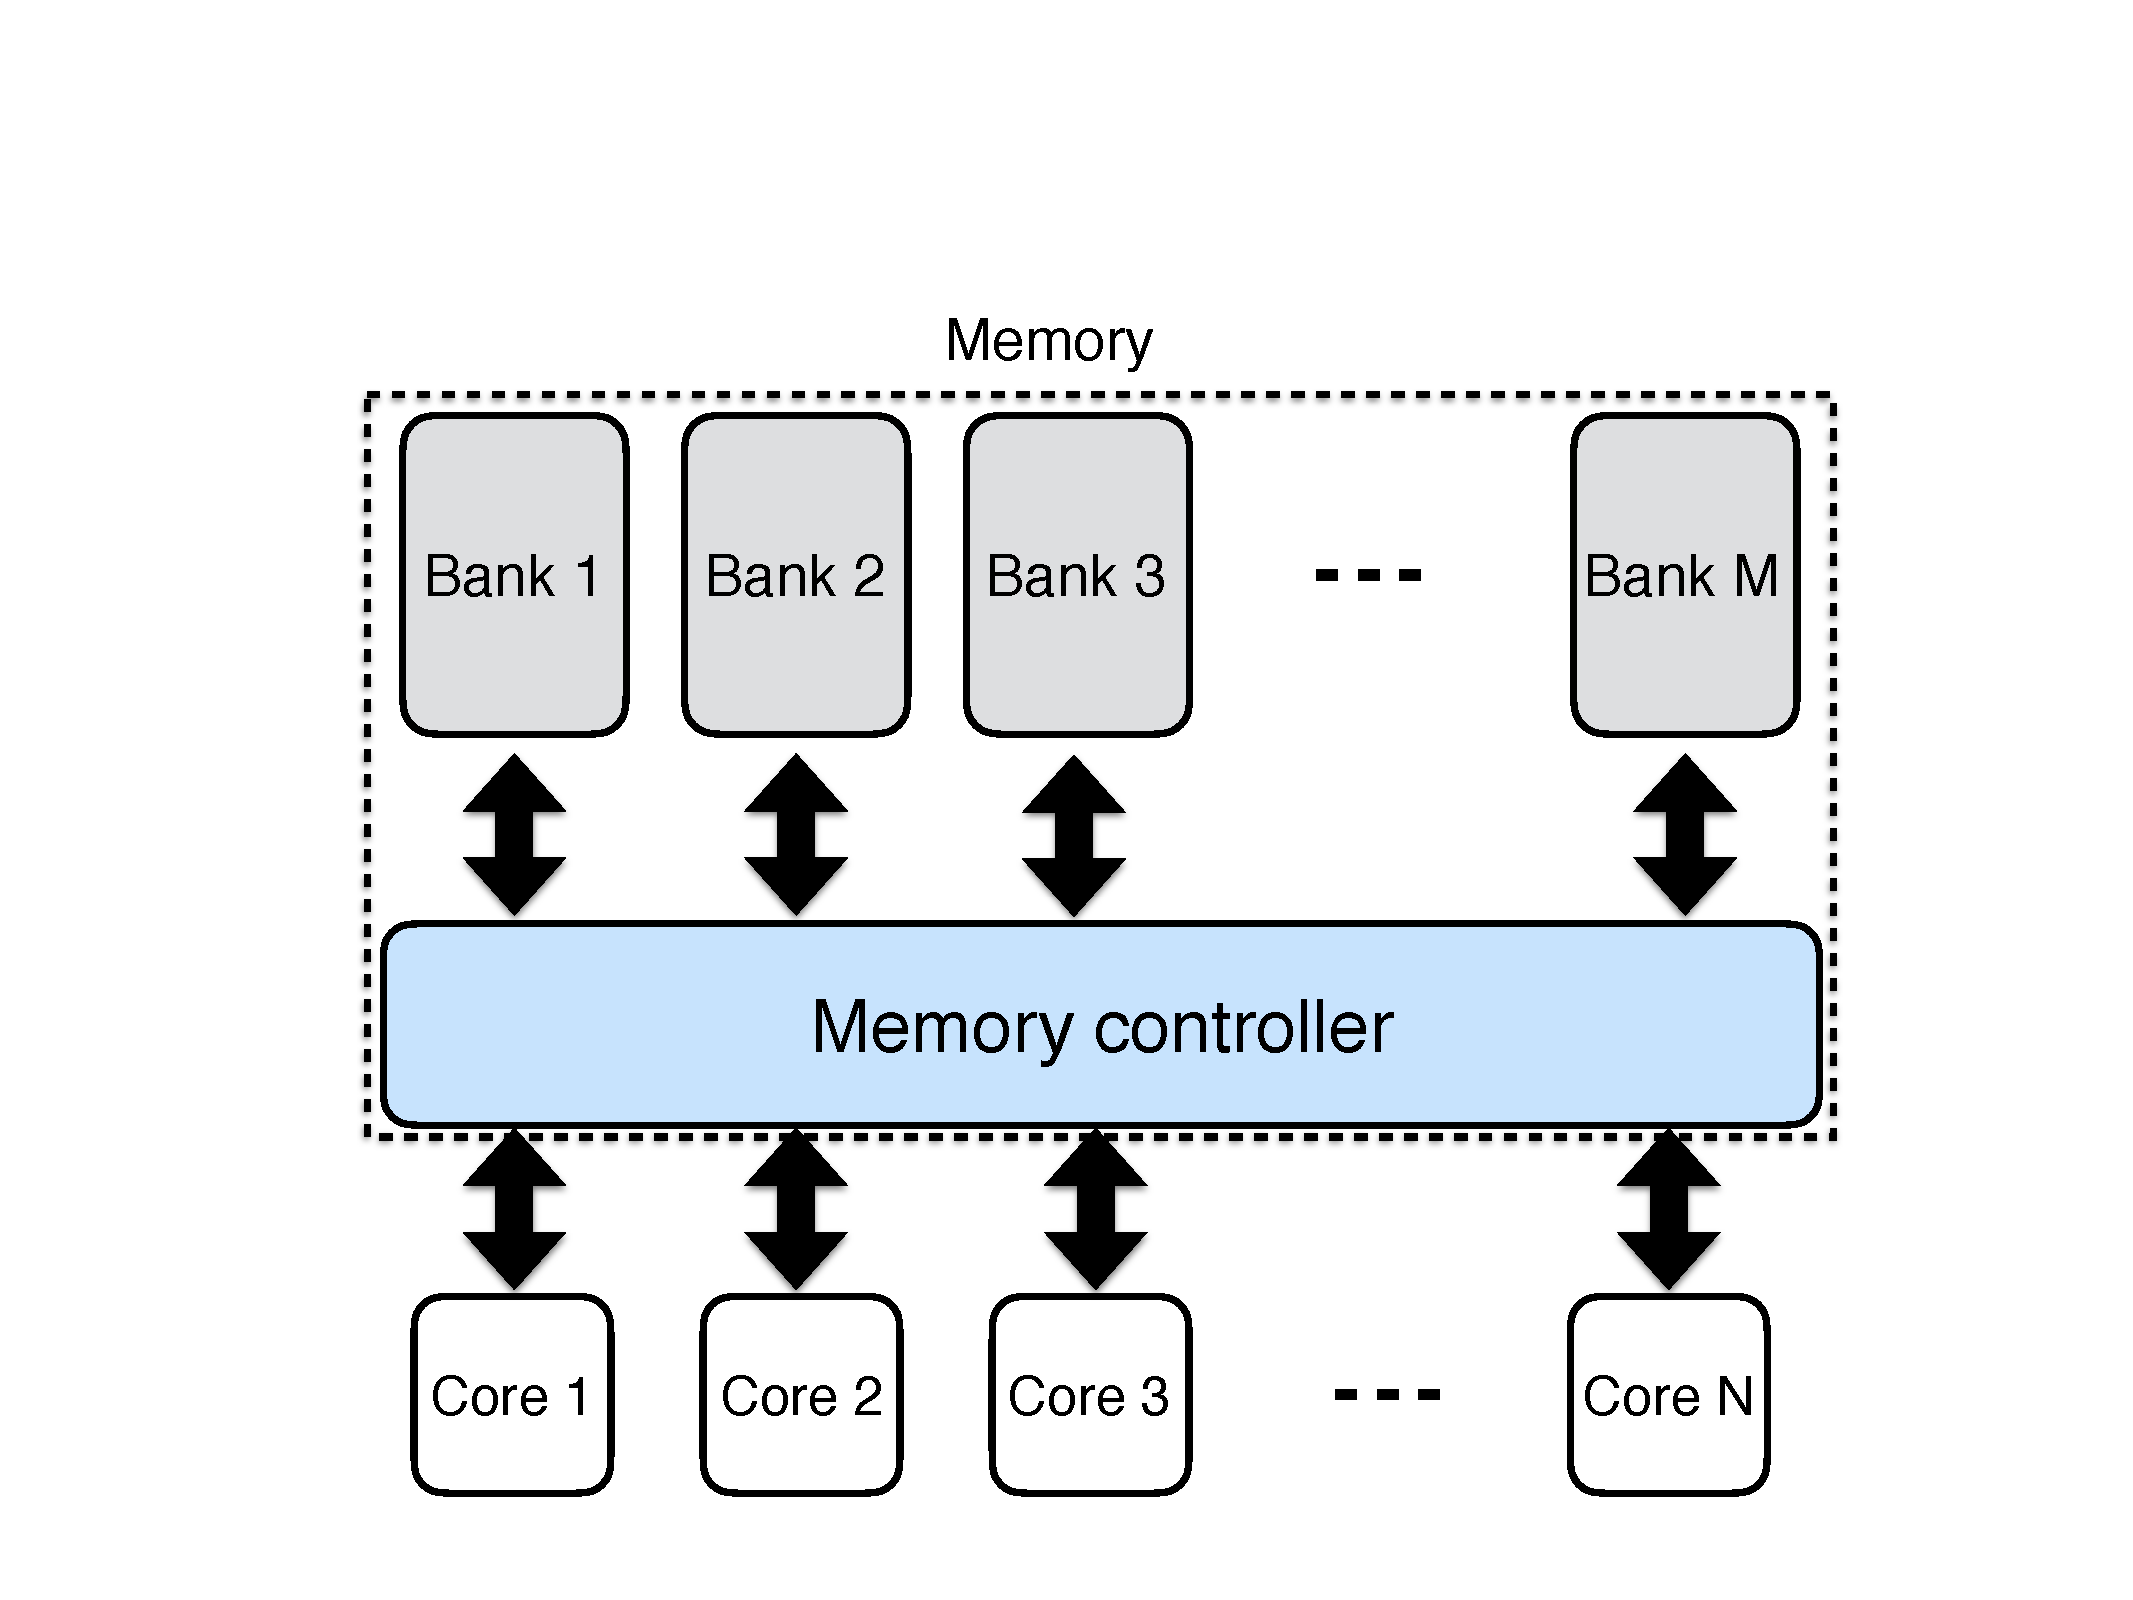
\includegraphics[width=0.85\linewidth]{figures/multicore-sys.pdf} 
\caption{Multi-core Architecture with shared memory.}
\label{fig:multicore}
\end{figure}
%%%%%%%%%%%%%%%%%%%%%%%%%%%%%%%%

 